% =====================================================================
%  SuperPC_2026 — documento principal
%  Compilar con:  make        (o)  latexmk -pdf main.tex
% =====================================================================
\documentclass[
  11pt,
  a4paper,
  oneside,
  spanish,
]{article}

% --- Configuracion (ver carpeta preamble/) -------------------------
% =====================================================================
%  preamble/packages.tex — paquetes y codificacion
% =====================================================================

% --- Codificacion e idioma ------------------------------------------
% Funciona con pdflatex. Si cambias a lualatex/xelatex, sustituye
% inputenc/fontenc por:  \usepackage{fontspec}
\usepackage[utf8]{inputenc}
\usepackage[T1]{fontenc}
\usepackage{babel}              % toma "spanish" de \documentclass
\usepackage{csquotes}           % requerido por babel + biblatex

% --- Tipografia ------------------------------------------------------
\usepackage{lmodern}
\usepackage{microtype}          % justificado y kerning mas finos

% --- Matematicas -----------------------------------------------------
\usepackage{amsmath, amssymb, amsthm}
\usepackage{mathtools}
\usepackage{siunitx}            % unidades: \SI{3.5}{\giga\hertz}
\sisetup{output-decimal-marker={,}, group-separator={.}}

% --- Figuras y tablas ------------------------------------------------
\usepackage{graphicx}
\graphicspath{{figures/}}
\usepackage{booktabs}           % tablas de calidad editorial
\usepackage{longtable}
\usepackage{tabularx}
\usepackage{multirow}
\usepackage{float}
\usepackage[labelfont=bf, font=small]{caption}
\usepackage{subcaption}

% --- Codigo fuente ---------------------------------------------------
\usepackage{listings}
\usepackage{caption}

% --- Varios ----------------------------------------------------------
\usepackage{enumitem}           % listas configurables
\usepackage{xspace}             % usado por las macros propias
\usepackage{eurosym}            % simbolo \euro
\usepackage{xcolor}
% todonotes es opcional: si no esta instalado, \todo y \revisar
% se vuelven silenciosos en vez de romper la compilacion.
% Para tener las notas al margen:
%   sudo dnf install 'tex(todonotes.sty)'
\IfFileExists{todonotes.sty}{%
  \usepackage{todonotes}%
}{%
  \newcommand{\todo}[2][]{}%
  \newcommand{\listoftodos}{}%
}

% --- Bibliografia ----------------------------------------------------
\usepackage[
  backend=biber,
  style=numeric,                % alternativas: authoryear, ieee, apa
  sorting=nty,
  maxbibnames=99,
]{biblatex}

% --- Hyperref SIEMPRE al final ---------------------------------------
\usepackage[
  hidelinks,
  pdfusetitle,
  breaklinks=true,
]{hyperref}
\usepackage{cleveref}           % \cref{...} despues de hyperref
   % paquetes y codificacion
% =====================================================================
%  preamble/style.tex — margenes, encabezados y apariencia
% =====================================================================

% --- Geometria de pagina ---------------------------------------------
\usepackage[
  a4paper,
  top=2.5cm, bottom=2.5cm,
  left=3cm,  right=2.5cm,
  headheight=14pt,
]{geometry}

% --- Espaciado -------------------------------------------------------
\usepackage{setspace}
\onehalfspacing
\setlength{\parskip}{0.5em}

% --- Encabezados y pies ----------------------------------------------
\usepackage{fancyhdr}
\pagestyle{fancy}
\fancyhf{}
\fancyhead[L]{\small\nouppercase{\leftmark}}
\fancyhead[R]{\small\thepage}
\renewcommand{\headrulewidth}{0.4pt}

% --- Paleta de color -------------------------------------------------
\definecolor{acento}{HTML}{1F4E79}
\definecolor{grisclaro}{HTML}{F5F5F5}
\definecolor{comentario}{HTML}{6A737D}

% --- Titulos de seccion ----------------------------------------------
\usepackage[explicit]{titlesec}
\titleformat{\section}
  {\Large\bfseries\color{acento}}{\thesection}{1em}{#1}
\titleformat{\subsection}
  {\large\bfseries}{\thesubsection}{1em}{#1}
\titlespacing*{\section}{0pt}{2.5ex plus 1ex minus .2ex}{1.5ex plus .2ex}

% --- Estilo de los bloques de codigo ---------------------------------
\lstdefinestyle{base}{
  backgroundcolor=\color{grisclaro},
  commentstyle=\color{comentario}\itshape,
  keywordstyle=\color{acento}\bfseries,
  stringstyle=\color{teal},
  basicstyle=\ttfamily\footnotesize,
  numberstyle=\tiny\color{comentario},
  numbers=left,
  numbersep=8pt,
  breaklines=true,
  breakatwhitespace=false,
  showstringspaces=false,
  tabsize=2,
  frame=single,
  rulecolor=\color{comentario!40},
  captionpos=b,
  extendedchars=true,
  literate=%
    {á}{{\'a}}1 {é}{{\'e}}1 {í}{{\'i}}1 {ó}{{\'o}}1 {ú}{{\'u}}1
    {Á}{{\'A}}1 {É}{{\'E}}1 {Í}{{\'I}}1 {Ó}{{\'O}}1 {Ú}{{\'U}}1
    {ñ}{{\~n}}1 {Ñ}{{\~N}}1 {ü}{{\"u}}1 {¿}{{?`}}1 {¡}{{!`}}1
}
\lstset{style=base}

% --- Entornos de teorema --------------------------------------------
\theoremstyle{definition}
\newtheorem{definicion}{Definicion}[section]
\newtheorem{ejemplo}{Ejemplo}[section]

\theoremstyle{plain}
\newtheorem{teorema}{Teorema}[section]
\newtheorem{lema}[teorema]{Lema}

\theoremstyle{remark}
\newtheorem*{nota}{Nota}
      % margenes, encabezados, colores
% =====================================================================
%  preamble/macros.tex — comandos propios del documento
%  Define aqui cualquier atajo para no repetir formato en el texto.
% =====================================================================

% --- Terminos recurrentes --------------------------------------------
% Uso: \pc{} escribe siempre el nombre igual en todo el documento.
\newcommand{\pc}{\textsc{SuperPC 2026}\xspace}

% --- Hardware / unidades --------------------------------------------
% Uso: \comp{Ryzen 9 9950X}  -> resalta un componente
\newcommand{\comp}[1]{\textbf{#1}}
% Uso: \precio{1250}         -> 1.250 EUR con formato consistente
\newcommand{\precio}[1]{\num{#1}\,\euro}

% --- Rutas, comandos y archivos -------------------------------------
\newcommand{\archivo}[1]{\texttt{#1}}
\newcommand{\cmd}[1]{\texttt{\textcolor{acento}{#1}}}

% --- Atajos matematicos ---------------------------------------------
\newcommand{\R}{\mathbb{R}}
\newcommand{\N}{\mathbb{N}}
\DeclareMathOperator*{\argmax}{arg\,max}
\DeclareMathOperator*{\argmin}{arg\,min}

% --- Marcadores de trabajo pendiente --------------------------------
% Uso: \revisar{falta la fuente de alimentacion}
\newcommand{\revisar}[1]{\todo[inline, color=yellow!40]{REVISAR: #1}}

     % comandos propios

% --- Datos de portada ---------------------------------------
\title{Instalación de RockyLinux e Instalación de OpenHPC para el Levantamiento de un Cluster}
\author{Lopez Lopez Mauricio Naim (355031)\\Silos Villegas Francisco Javier (333127)\\Muñoz Amaro Guillermo Jair (332508)\\Rodríguez Torres Jacobo (351022)
}

\date{
    Ingeniería en Sistemas Inteligentes\\
    Ingeniería en Computación\\[1em] 
    Generación 2022\\[1em]
    Clave de la facultad: 202202300179\\[1em]
    Supercómputo\\
    Grupo 222801\\
    \today
  }

\addbibresource{bib/referencias.bib}

% =====================================================================
\begin{document}

\maketitle
\thispagestyle{empty}

\clearpage
\tableofcontents
\clearpage

\section{Resumen}
\label{sec:resumen}

Problema
Se tiene la necesidad de la creación de un cluster para poder realizar cómputo en paralelo a través de este mismo, una red local privada y una red pública para que un cliente pueda conectarse al nodo maestro y así cargar o ejecutar su programa dentro del cluster, de esta forma conseguir que se ejecute correctamente y asegurar el funcionamiento correcto de el mismo.

\subsection{Objetivos}

\begin{itemize}[noitemsep]
  \item Instalar software para maquinas virtuales (VBox/KVM)
  \item Instalar RockyLinux 10
  \item Instalar OpenHPC y sus componentes necesarios
  \item Establecer topología de red pública y privada para el Cluster y su tabla de direccionamiento 
  \item Crear nodo maestro y crear 3 nodos de cómputo
  \item Realizar pruebas de hola mundo
\end{itemize}

\subsection{Métodos empleados}

Instalación del sistema operativo base usando la guía oficial de rocky linux para poder ejecutarla en una máquina virtual de Virtualbox. Una vez completado esto, se sigue la serie de pasos del manual de instalación de OpenHPC.
Adicionalmente se instala y configura warewulf y se instala y configura slurm, finalmente se instaló un servidor Network Time Protocol

\subsection{Resultados}

\subsection{Conclusiones principales}


\section{Contenido}
\label{sec:contenido}

Para poder hacer un cluster y hacer funcionar la red se tiene pensado implementar la guía de OpenHPC para su versión 4.1, cabe recalcar que en todo momento se ejecutan los comandos de la guía en modo root o privilegiado, a no ser que se indique lo contrario. Se asume que para la instalación haciendo uso de la guía hay disponibilidad para un equipo que sea nodo maestro y 3 equipos que sean nodos de cómputo, el nodo maestro funciona como un system management server (SMS) en el cuál tiene instalado RockyLinux 10.

\subsection{Topología de red y tabla de direccionamiento}
La topología que se va a plantear cuenta con dos partes, la red pública y la red privada, en donde el cliente va a ser capaz de conectarse vía ssh con la red pública al nodo maestro para poder cargar su programa y el nodo maestro se encargará de distribuir la carga de este a través de la red privada.
\\[1em]
La topología propuesta gráficamente es la siguiente:
\begin{figure}[H]
  \centering
  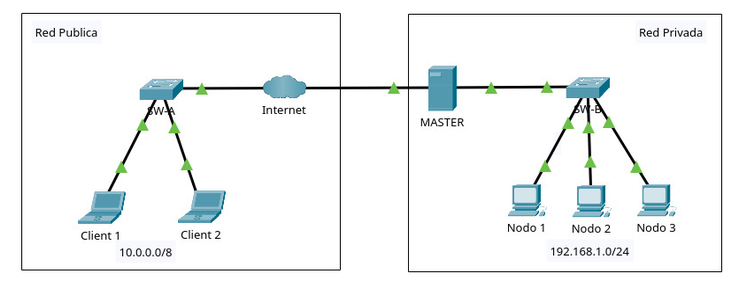
\includegraphics[width=0.9\textwidth]{topologia1}
  \caption{Topología de red propuesta con la red pública y la red privada}
  \label{fig:topologia}
\end{figure}

La tabla de direccionamiento propuesta es la siguiente:
\begin{table}[H]
  \centering
  \caption{Tabla de direccionamiento propuesta para la red privada y pública}
  \label{tab:direccionamiento}
  \begin{tabular}{llll}
    \toprule
    \textbf{Dispositivos} & \textbf{Interfaz} & \textbf{Dirección IPv4} & \textbf{Máscara de subred} \\
    \midrule
    MASTER    & NIC 1 & \texttt{192.168.1.10} & \texttt{255.255.255.0} \\
    Nodo 1    & NIC   & \texttt{192.168.1.11} & \texttt{255.255.255.0} \\
    Nodo 2    & NIC   & \texttt{192.168.1.12} & \texttt{255.255.255.0} \\
    Nodo 3    & NIC   & \texttt{192.168.1.13} & \texttt{255.255.255.0} \\
    \midrule
    MASTER    & NIC 2 & \texttt{10.0.0.10}    & \texttt{255.0.0.0} \\
    Cliente 1 & NIC   & \texttt{10.0.0.11}    & \texttt{255.0.0.0} \\
    Cliente 2 & NIC   & \texttt{10.0.0.12}    & \texttt{255.0.0.0} \\
    Cliente N & NIC   & \texttt{10.0.0.13}    & \texttt{255.0.0.0} \\
    \bottomrule
  \end{tabular}
\end{table}


\subsection{Instalación de RockyLinux 10}
Para la instalación de RockyLinux 10 es requerido para este proyecto hacer uso de máquinas virtuales, en este caso usaremos diferentes aplicaciones de máquinas virtuales como KVM y VMBox, para este caso se instalará RockyLinux con interfaz, se asume que el software de virtualización para las máquinas virtuales ya está instalado y únicamente se tiene que configurar la instalación del sistema operativo (SO). Para ello, nos dirigimos a la página oficial de rocky Linux para poder descargar la imagen ISO correspondiente, la versión utilizada para este caso es la 10.2 DVD ISO, una vez descargada se crea la máquina virtual en VirtualBox.
\\[1em]
\begin{figure}[H]
  \centering
  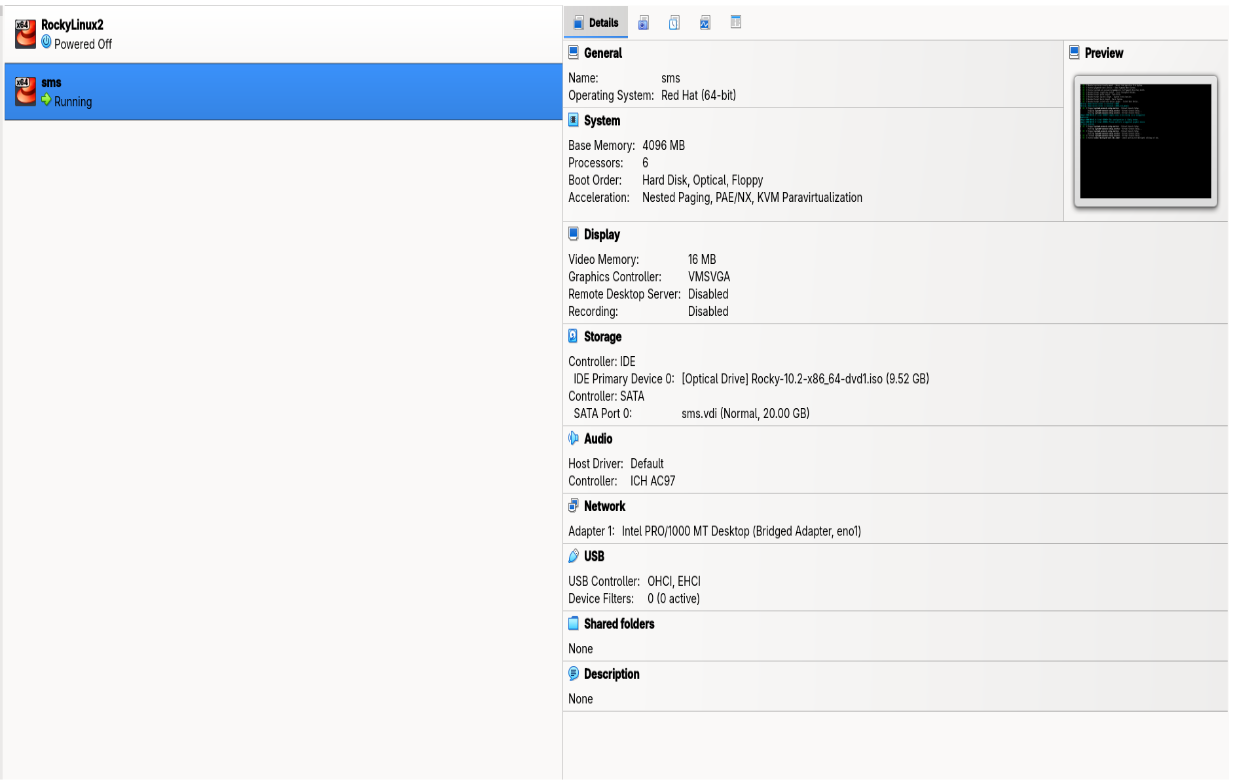
\includegraphics[width=0.9\textwidth]{maquinaVirtual2}
  \caption{Máquina virtual del nodo maestro creada en VirtualBox}
  \label{fig:vm-virtualbox}
\end{figure}

Una vez creada la máquina con 4GB de RAM y 4 núcleos de procesamiento asignados se procede a la instalación por defecto del sistema operativo (SO).

\begin{figure}[H]
  \centering
  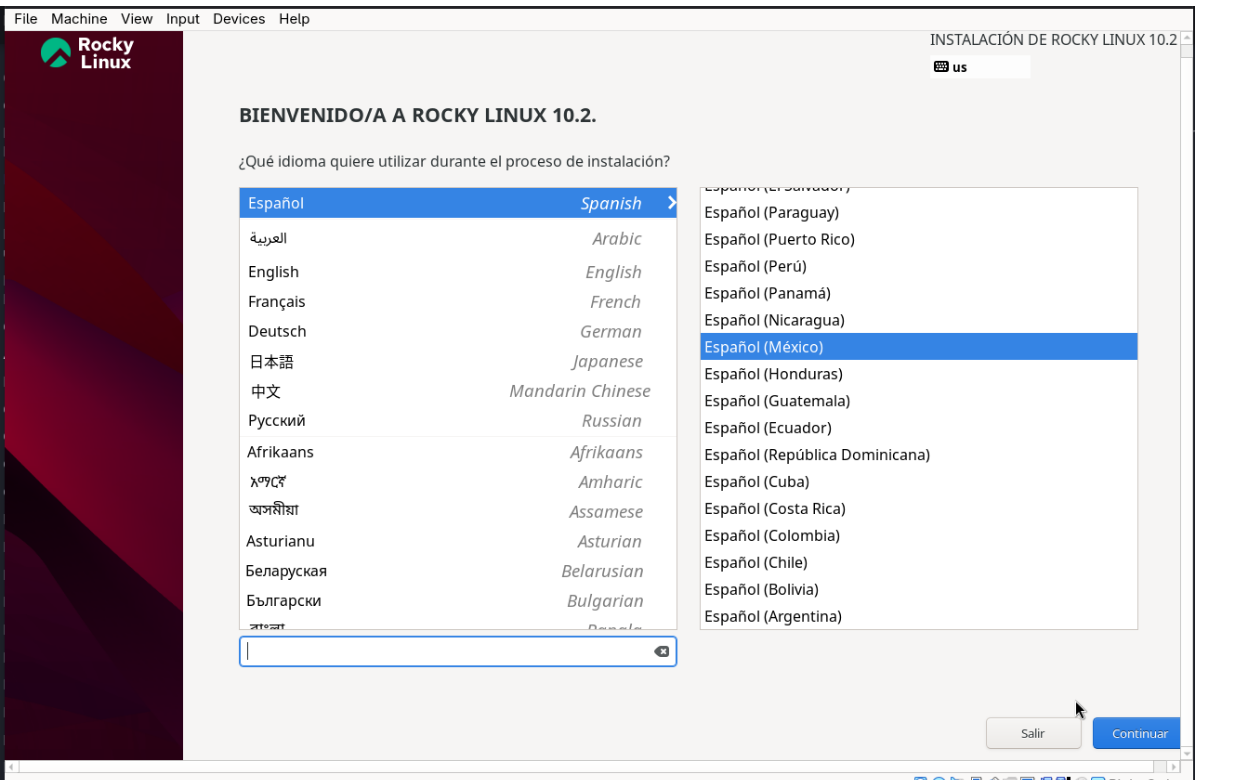
\includegraphics[width=0.9\textwidth]{RockyLinux3}
  \caption{Selección de idioma al iniciar la instalación de Rocky Linux 10.2}
  \label{fig:rocky-idioma}
\end{figure}

Con la máquina virtual iniciada por primera vez, lo primero que se hizo fue la instalación base, una vez seleccionados los parámetros de instalación se finalizó la instalación y comienza la configuración de OpenHPC para el nodo maestro.

\begin{figure}[H]
  \centering
  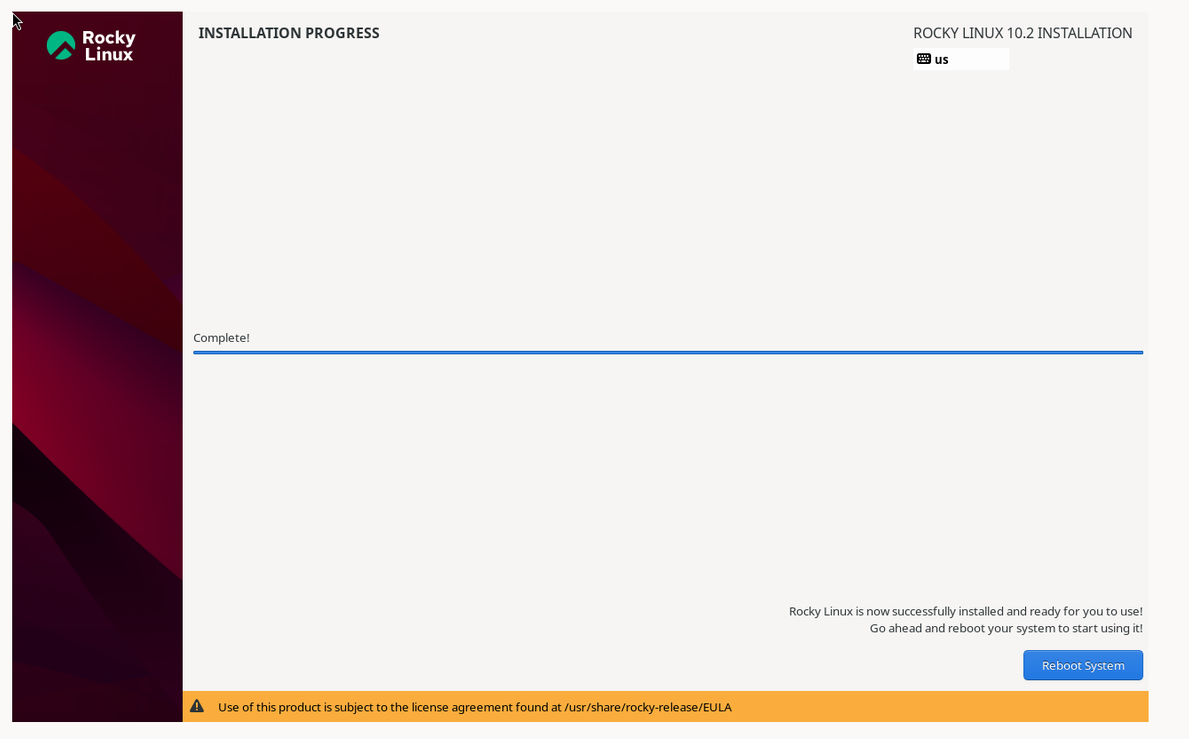
\includegraphics[width=0.9\textwidth]{RockyLinux4}
  \caption{Instalación del sistema operativo base finalizada}
  \label{fig:rocky-instalado}
\end{figure}

Posterior a la instalación del sistema operativo base (BOS) se deshabilita SELinux ya que así lo requiere la instalación guiada del manual de OpenHPC.


\begin{figure}[H]
  \centering
  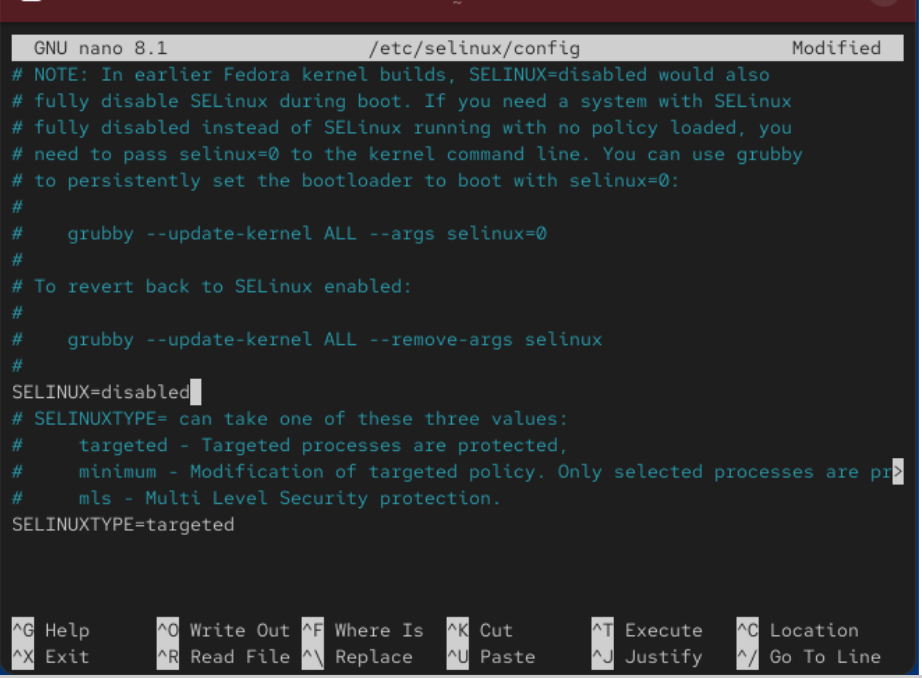
\includegraphics[width=0.9\textwidth]{SElinux5}
  \caption{SELinux deshabilitado en \texttt{/etc/selinux/config}}
  \label{fig:selinux}
\end{figure}

Se habilitan los repositorios de paquetes EL, ya que el nodo maestro requiere que se tengan los repositorios estándar del BOS para tener acceso a paquetes como BaseOS, Appstream, Extras, CRB y EPEL, de esta forma se puede tener acceso remoto a estos repositorios y permitir avanzar con la instalación, haciendo uso de los siguientes comandos es posible hacer esto:

\begin{lstlisting}[language=bash, caption={Comandos para habilitar paquetes EL}, label={lst:epel}]
$ sudo dnf -y install epel-release dnf-plugins-core
$ sudo dnf config-manager --set-enabled crb
\end{lstlisting}

\subsection{Configuración del firewall}
Para poder obtener acceso a través de los protocolos de HTTP, DHCP y TFTP se tiene que deshabilitar el firewall manualmente en el BOS del nodo maestro ya que si no no podrá tener comunicación y prohibición con estos servicios.
\\[1em]
Para deshabilitar se hace uso del siguiente comando:
\begin{lstlisting}[language=bash, caption={Comando para desactivación de firewall}, label={lst:firewall}]
$ systemctl disable --now firewalld || true
\end{lstlisting}
\subsection{Configuración de NTP}
Los sistemas HPC dependen de una sincronización del reloj en sus nodos a través del protocolo de NTP para facilitar su sincronización, se habilitó NTP en el nodo maestro y a su vez el nodo maestro es el servidor de NTP con el siguiente comando:

\begin{lstlisting}[language=bash, caption={Comandos para configurar el servidor NTP}, label={lst:ntp}]
$ sudo dnf -y install chrony
$ sudo systemctl enable chronyd.service
$ sudo echo "local stratum 10" >> /etc/chrony.conf
$ sudo echo "server 192.168.1.10" >> /etc/chrony.conf
$ sudo echo "allow all" >> /etc/chrony.conf
$ sudo systemctl restart chronyd 
\end{lstlisting}
En este caso, el manual especifica opcionalmente instalar infiniBand y Omnipath, sin embargo no tenemos la necesidad ya que no manejaremos un ancho de banda muy grande (arriba de \SI{1}{\giga\bit\per\second}).

\subsection{Instalación de componentes OpenHPC (OHPC)}
En primer instancia habilitamos el repositorio de OHPC haciendo uso del siguiente comando:

\begin{lstlisting}[language=bash, caption={Comando para habilitar el repositorio de OHPC}, label={lst:ohpc-repo}]
$ sudo dnf -y install http://repos.openhpc.community/OpenHPC/4/EL_10/x86_64/ohpc-release-4-1.el10.x86_64.rpm
\end{lstlisting}

Posteriormente se instalan los paquetes de OHPC con el siguiente comando

\begin{lstlisting}[language=bash, caption={Comando para instalar los paquetes base de OHPC}, label={lst:ohpc-base}]
$ sudo dnf -y install ohpc-base
\end{lstlisting}  

\subsection{Instalación de Slurm en el nodo maestro}
Slurm es el manejador de recursos para el cluster, este es necesario para que se pueda hacer uso de los nodos y este estará instalado en el nodo maestro, haciendo uso de los siguientes comandos tenemos la instalación de este:

\begin{lstlisting}[language=bash, caption={Comandos para instalar Slurm}, label={lst:slurm-server}]
# Instalación del paquete de servidor de Slurm
$ sudo dnf -y install ohpc-slurm-server
# Configuración de Slurm a través del archivo otorgado por ohpc
$ cp /etc/slurm/slurm.conf.ohpc /etc/slurm/slurm.conf
# Configuración de los cgroup
$ cp /etc/slurm/cgroup.conf.example /etc/slurm/cgroup.conf
# Identificación del nodo maestro en el servidor de Slurm
$ sudo sed -i "s/SlurmctldHost=\S\+/SlurmctldHost=${sms_name}/" \
/etc/slurm/slurm.conf
\end{lstlisting}  

\subsection{Instalación de warewulf en el nodo maestro}
Para poder hacer uso de warewulf, el cuál es esencial para la instalación del cluster para proveer los paquetes necesarios a los nodos de cómputo, hacemos uso de los siguientes comandos:

\begin{lstlisting}[language=bash, caption={Comandos para instalación de warewulf}, label={lst:warewulf}]
$ sudo dnf -y install warewulf-ohpc yq
$ sudo install -d -m 0755 /var/lib/tftpboot
\end{lstlisting}  
Posterior a la instalación, es necesario realizar modificaciones en los archivos de configuración de warewulf, usando los siguientes comandos se establece todo lo necesario para ello:

\begin{lstlisting}[language=bash, caption={Comandos para modificar archivos de configuración de warewulf}, label={lst:warewulf-conf}]
$ sudo yq -i '.ipaddr = "'"${sms_ip}"'"' /etc/warewulf/warewulf.conf
$ sudo yq -i '.netmask = "'"${internal_netmask}"'"' /etc/warewulf/warewulf.conf
$ sudo yq -i '.network = "'"${internal_network}"'"' /etc/warewulf/warewulf.conf
$ sudo yq -i '.dhcp["range start"] = "'"${internal_network}"'"' \
/etc/warewulf/warewulf.conf
$ sudo yq -i '.dhcp["range end"] = "static"' /etc/warewulf/warewulf.conf
$ sudo yq -i '.dhcp.template = "static"' /etc/warewulf/warewulf.conf
$ sudo sed -i "s/defaults,noauto,nofail,ro/defaults,nofail,ro/" \
/etc/warewulf/nodes.conf
$ sudo yq -i '.nodeprofiles.default.kernel.args -= ["quiet"]' \
/etc/warewulf/nodes.conf
$ sudo echo "log-debug" >> /etc/dnsmasq.d/ww4-debug.conf
$ sudo systemctl enable --now warewulfd
$ sudo wwctl profile add nodes --profile default --comment "Nodes profile"
$ sudo wwctl overlay create nodeconfig
$ sudo wwctl profile set --yes nodes --system-overlays nodeconfig \
--runtime-overlays syncuser
$ sudo wwctl profile set -y nodes --netname=default --netdev="${eth_provision}"
$ sudo wwctl profile set -y nodes --netname=default --netmask="${internal_netmask}"
$ sudo wwctl profile set -y nodes --netname=default --gateway="${ipv4_gateway}"
$ sudo wwctl profile set -y nodes --netname=default --nettagadd=DNS="${dns_servers}"
$ sudo wwctl configure --all
$ bash /etc/profile.d/ssh_setup.sh
\end{lstlisting} 

\subsection{Creación de la imagen del nodo de cómputo}
Para este paso crearemos una imagen mínima para el nodo de cómputo, esto se tiene que hacer con el objetivo de que se use con warewulf ya que tiene que incluir el kernel y un sistema init, con los siguientes comandos, esto es posible de realizar:
\\
Importar la imagen base para warewulf:
\begin{lstlisting}[language=bash, caption={Comando para importar la imagen del nodo de cómputo}, label={lst:imagen-import}]
$ sudo wwctl image import docker://ghcr.io/warewulf/warewulf-rockylinux:10 \
rocky-10 --syncuser
\end{lstlisting}  

Posterior a esto, los siguientes comandos son en el nodo de cómputo:

\begin{lstlisting}[language=bash, caption={Comandos para configurar el nodo de cómputo}, label={lst:imagen-config}]
# Establecer el CHROOT 
$ sudo CHROOT=$(wwctl image show rocky-10)
export CHROOT
# Habilitar OHPC y deshabilitar el reinicio en cada ejecución
$ sudo wwctl image exec --build=false rocky-10 -- /bin/bash -ex <<- EOF
$ sudo dnf -y install dnf-utils
$ sudo dnf -y install http://repos.openhpc.community/OpenHPC/4/EL_10/\
x86_64/ohpc-release-4-1.el10.x86_64.rpm
$ sudo dnf -y update
\end{lstlisting}  

\subsection{Agregar componentes de OHPC}
Ahora se necesitan recursos adicionales para el servicio de NTP, soporte del cliente y otros paquetes adicionales necesarios para soportar OHPC. Con los siguientes comandos esto es posible:

\begin{lstlisting}[language=bash, caption={Comando de componentes adicionales de OHPC en el nodo maestro}, label={lst:ohpc-maestro}]
$ sudo wwctl image exec --build=false rocky-10 -- /bin/bash -ex
\end{lstlisting}  
Los siguientes comandos son en el nodo de cómputo
\begin{lstlisting}[language=bash, caption={Comando de componentes adicionales de OHPC en el nodo de cómputo}, label={lst:ohpc-computo}]
$ sudo dnf -y install epel-release
$ sudo dnf -y install ohpc-base-compute
# Agregar Slurm al cliente
dnf -y install ohpc-slurm-client
# habilitar que los servicios se inicien al arrancar
systemctl enable munge.service
systemctl enable slurmd.service
# Agregar NTP para sincronización
dnf -y install chrony
# Incluir modulos de OHPC
dnf -y install lmod-ohpc
\end{lstlisting}  

\subsection{Importar archivos}
El sistema de warewulf tiene ciertos archivos que son necesariamente deben de estar compartidos a lo largo de los nodos de cómputo, para realizar esto se usan los siguientes comandos y se aplican en todos los nodos de cómputo:


\begin{lstlisting}[language=bash, caption={Comandos de importación de archivos}, label={lst:overlay-import}]
$ sudo wwctl overlay import --parents nodeconfig /etc/subuid
$ sudo wwctl overlay import --parents nodeconfig /etc/subgid
$ sudo wwctl overlay import --parents nodeconfig \
/opt/ohpc/pub/examples/chrony.conf.ww /etc/chrony.conf.ww
$ sudo wwctl profile set --yes nodes --tagadd ntpserver="${sms_ip}"
$ sudo wwctl overlay import --parents nodeconfig \
/opt/ohpc/pub/examples/network/NetworkManager-wait-online.service.d/override.conf \
/etc/systemd/system/NetworkManager-wait-online.service.d/override.conf
\end{lstlisting} 

\subsection{Configuración de Slurm}
Para configurar Slurm e importar las claves criptográficas necesitamos autenticación de munge para que esté disponible en todos los hosts, usando los siguientes comandos configuramos este apartado:

\begin{lstlisting}[language=bash, caption={Comandos de configuración de Slurm en el nodo de cómputo}]
# Configurar el servidor de Slurm
$ sudo wwctl overlay import --parents nodeconfig \
/opt/ohpc/pub/examples/slurm/slurmd.ww /etc/sysconfig/slurmd.ww
# Asignar el valor del slurmctl al nodo maestro
$ sudo wwctl profile set --yes nodes --tagadd slurmctld="${sms_ip}"
# Configurar munge
$ sudo wwctl overlay import --parents nodeconfig /etc/munge/munge.key
$ sudo wwctl overlay chown nodeconfig /etc/munge/munge.key \
"$(id -u munge)" "$(id -g munge)"
$ sudo wwctl overlay chown nodeconfig /etc/munge "$(id -u munge)" "$(id -g munge)"
$ sudo wwctl overlay chmod nodeconfig /etc/munge 0700
\end{lstlisting}

\subsection{Pasos finales de configuración}
\subsubsection{Levantar imágenes y overlays}
Se habilita el levantamiento de dracut y la imagen ya que en pasos anteriores lo teníamos deshabilitado, de esta forma se vuelve a levantar la imagen con configuraciones nuevas posibles, esto con los siguientes comandos:

\begin{lstlisting}[language=bash, caption={Comandos para habilitar levantamiento de dracut}]
#Levantar los inits de dracut
$ sudo wwctl image exec --build=false rocky-10 -- /usr/bin/dracut --force \
--regenerate-all
# Levantar la imagen
$ sudo wwctl image build rocky-10
$ sudo wwctl overlay build  
\end{lstlisting}

\subsubsection{Habilitar control con ssh vía administrador de recursos}
Restringimos el acceso a ssh directamente en los nodos de cómputo, esto con el objetivo de que solo se puedan acceder desde el nodo maestro o usuarios que tienen una tarea activa en el nodo, esto lo hicimos con un simple comando:

\begin{lstlisting}[language=bash, caption={Comando para habilitar ssh por medio del nodo maestro}]
$ sudo echo 'account required pam_slurm.so'  >> "$CHROOT/etc/pam.d/sshd"  
\end{lstlisting}

\subsection{Herramientas del administrador en el cluster}
\subsubsection{Agregar ClusterShell}
Como su nombre lo dice, agregamos un shell para poder ejecutar tareas en paralelo en los nodos de cómputo con los siguientes comandos:

\begin{lstlisting}[language=bash, caption={Comando para instalar clustershell y definiciones de nodos}]
  # Instalar el clustershell
$ sudo dnf -y install clustershell
# Definir definiciones de los nodos
$ mv /etc/clustershell/groups.d/local.cfg \
/etc/clustershell/groups.d/local.cfg.orig
$ sudo echo "adm: sms" > \
/etc/clustershell/groups.d/local.cfg
$ sudo echo "compute: computeprefix[1-3]" >> \
/etc/clustershell/groups.d/local.cfg
$ sudo echo "all: @adm,@compute" >> /etc/clustershell/groups.d/local.cfg
\end{lstlisting}

\subsubsection{Agregar NHC}
Node health check sirve para que podamos visualizar el estado de los nodos de cómputo, y de esta forma verificar si es que están funcionando correctamente o no, a su vez se pueden marcar los nodos como “unhealthy” para poder saber que no están conectados o algo no está bien en ellos, esto con los siguientes comandos:

\begin{lstlisting}[language=bash, caption={Comandos para instalar y configurar NHC}]
# Instalar NHC en el nodo maestro y en los nodos de cómputo
$ sudo dnf -y install nhc-ohpc
$ sudo dnf -y --installroot="$CHROOT" install nhc-ohpc
# Registrarlo como parte de Slurm
$ sudo echo "HealthCheckProgram=/usr/sbin/nhc" >> /etc/slurm/slurm.conf
# Revisar el estado cada 5 minutos o 300 segundos
$ sudo echo "HealthCheckInterval=300" >> /etc/slurm/slurm.conf  
\end{lstlisting}

\subsection{Despliegue del cluster}
Los nodos de cómputo se registran en base a un ciclo de comandos con la siguiente instrucción:

\begin{lstlisting}[language=bash, caption={Comandos en ciclo para registrar nodos de cómputo}] 
$ for ((i=0; i<num_computes; i++)) ; do
  wwctl node add --image=rocky-10 --profile=nodes --netname=default \
    --ipaddr="${c_ip[$i]}" --hwaddr="${c_mac[$i]}" "${c_name[i]}"
done
\end{lstlisting}

Finalmente actualizamos y recompilamos los overlays y actualizamos la configuración de warewulf con los siguientes comandos:

\begin{lstlisting}[language=bash, caption={Comandos para actualizar y recompilar warewulf}]
# Recompilado de la imagen de Rocky10
$ wwctl image build rocky-10
# compilar los overlays para todos los nodos de cómputo
$ wwctl overlay build
# Actualizar warewulf y su configuración
$ wwctl configure --all
\end{lstlisting}

\subsection{Inicializar Slurm}
Una vez funcionando Warewulf y los nodos de cómputo, podemos inicializar Slurm para poder administrar sus recursos y así poder permitirle al usuario hacer sus tareas, trabajos, programas, etc.
Esto con los siguiente comandos:

\begin{lstlisting}[language=bash, caption={Comandos para inicializar Slurm}]
$ systemctl enable --now munge
$ systemctl enable --now slurmctld
\end{lstlisting}

\subsection{Arrancar nodos de cómputo}
Para este punto, el nodo maestro ya es capaz de arrancar los nodos de cómputo, asumimos que los nodos de cómputo están configurados por BIOS con la opción de arranque por ethernet, con los siguientes comandos usando ipmitool iniciamos los hosts deseados en un ciclo de comandos, para poder hacer este una variable de entorno \texttt{IPMI\_PASSWORD} tiene que estar previamente configurada con la contraseña local BMC para poder así interactuar, las instrucciones en ciclo son las siguientes:

\begin{lstlisting}[language=bash, caption={Ciclo de comandos para arrancar los nodos de cómputo}]
$ for ((i=0; i<num_computes; i++)) ; do
    ipmitool -E -I lanplus -H "${c_bmc[$i]}" -U "${bmc_username}" \
      -P "${bmc_password}" chassis power reset
  done
\end{lstlisting}

Una vez terminado el proceso de booteo, toma menos de 5 minutos dependiendo de la BIOS pero se puede verificar que esto funcionó a través de una sesión de ssh o herramientas paralelas de ssh para múltiples hosts, para correr un comando en un nodo recién booteado se puede usar pdsh con el siguiente comando:

\begin{lstlisting}[language=bash, caption={Comando para probar un nodo recién booteado}]
$ pdsh -w ${compute_prefix}[1-${num_computes}] uptime  
\end{lstlisting}

Con este ejecutado nos arrojará información de los nodos de cómputo que tenga booteados

\subsection{Instalación de componentes de OHPC para desarrollo}

Los siguientes paquetes de instalación son para poder dar soporte a compiladores y herramientas de desarrollo como C/C++/FORTRAN en los nodos, pilas de MPI y otra variedad de bibliotecas de terceros

\subsubsection{Herramientas de desarrollo}

OpenHPC provee versiones de herramientas GNU como Valgrind, EasyBuild y Spack, se instalan con los siguientes comandos:
\begin{lstlisting}[language=bash, caption={Comandos para instalar herramientas GNU de OHPC}]
$ dnf -y install ohpc-autotools
$ dnf -y install EasyBuild-ohpc
$ dnf -y install hwloc-ohpc
$ dnf -y install spack-ohpc
$ dnf -y install valgrind-ohpc
\end{lstlisting}

\subsubsection{Compiladores}
OpenHPC a su vez, también da soporte de paquetes para compiladores GNU, estos se instalan con el siguiente comando:
\begin{lstlisting}[language=bash, caption={Comando para instalar compiladores GNU}]
$ sudo dnf -y install gnu15-compilers-ohpc
\end{lstlisting}

\subsubsection{Pilas MPI}
Para poder tener soporte de desarrollo y ejecución de MPI, OpenHPC también da soporte para esto con un paquete que provee variedad de usos de MPI y de capa de transporte, para este caso lo instalaremos para poder tener soporte del protocolo TCP con el siguiente comando:

\begin{lstlisting}[language=bash, caption={Comando para instalar pilas MPI}]
$ sudo dnf -y install openmpi5-pmix-gnu15-ohpc mpich-ofi-gnu15-ohpc
\end{lstlisting}

\subsubsection{Herramientas de rendimiento}
OpenHPC provee múltiples herramientas open-source para poder tener análisis de rendimiento, el grupo de herramientas se instala con el siguiente comando:
\begin{lstlisting}[language=bash, caption={Comando para instalar herramientas de análisis de rendimiento}]
$ sudo dnf -y install ohpc-gnu15-perf-tools
\end{lstlisting}

Finalmente se instala el entorno de desarrollo default que también convenientemente lo provee OpenHPC y además son módulos preconfigurados con el siguiente comando:
\begin{lstlisting}[language=bash, caption={Comando para instalar el entorno de desarrollo default}]
$ sudo dnf -y install lmod-defaults-gnu15-openmpi5-ohpc
\end{lstlisting}

\subsection{Post provisión}
Después de todas las instalaciones, hay que revisar el estado de los nodos con Slurm usando el comando sinfo, todos los nodos deberán de estar en "idle state" sin asterisco, si el estado se reporta como desconocido el siguiente comando puede cambiar el estado:

\begin{lstlisting}[language=bash, caption={Comando para cambiar el estado de un nodo a "idle"}]
$ scontrol update partition=normal state=idle
\end{lstlisting}

Ahora, para poder realizar pruebas con el cluster es necesario agregar un usuario que pueda correr un programa de prueba con el siguiente comando esto es posible, agregando al usuario "test":

\begin{lstlisting}[language=bash, caption={Comando para agregar un usuario de prueba}]
$ useradd -m test
\end{lstlisting}

Después de esto es necesario recompilar el overlay de WareWulf para su sincronización con los archivos en los nodos de cómputo con el siguiente comando:

\begin{lstlisting}[language=bash, caption={Comando para actualizar los archivos de los nodos de cómputo}]
$ wwctl overlay build
\end{lstlisting}

Por último tenemos que generar la configuración NHC basada en el entorno de los nodos de cómputo con el siguiente comando:

\begin{lstlisting}[language=bash, caption={Comando para crear la configuración de NHC}]
$ pdsh -w c1 "/usr/sbin/nhc-genconf -H '*' -c -" | dshbak -c
\end{lstlisting}

\subsection{Cluster Test}
Ahora que todo está listo, se hace una prueba con el cluster para asegurar su estado operacional, para esto usaremos un "hello world" ya incluido en los archivos de OpenHPC y las herramientas MPI previamente instaladas para que con un solo comando podamos hacer ejecución en paralelo en un entorno de OHPC, para hacer una sesión interactiva con el administrador de recursos se hace uso de los siguientes comandos:

\begin{lstlisting}[language=bash,caption={comandos para hacer un hola mundo de prueba con los nodos}]
# cambio al usuario test
su - test
# Compilar "hello world" de MPI en la carpeta de OHPC
[test@sms ~]$ mpicc -O3 /opt/ohpc/pub/examples/mpi/hello.c
# subir el archivo y usar prun para realizar la prueba interactiva
[test@sms ~]$ salloc -n 8 -N 2
[test@c1 ~]$ prun ./a.out 
\end{lstlisting}

Con todos estos comandos e instalación ya terminada la siguiente sección muestra hasta que punto llegamos y que resultados fueron los que obtuvimos.

\section{Resultados}
\label{sec:resultados}

Por la parte de los resultados que obtuvimos, pudimos hacer la instalación correcta del nodo maestro y los nodos de cómputo, desafortunadamente no pudimos terminar a tiempo la prueba del hola mundo debido a que tuvimos un problema con el servidor de DHCP, la red y los nodos, por alguna razón al iniciar las maquinas virtuales esperando booteo por ethernet, el nodo maestro les ofrecía la dirección que le tocaba a cada equipo pero sin tener éxito en esta negociación ya que el equipo de los nodos rechazaban la dirección, incluso forzandolo y manualmente estableciendo la dirección ip en cada equipo no obtuvimos arranque con la imagen de Rocky 10 por ethernet, tiempo después si fuimos capaces de conseguir que se asignaran las ips y finalmente arrancaran por booteo de ethernet, estos son los resultados:

\begin{figure}[H]
  \centering
  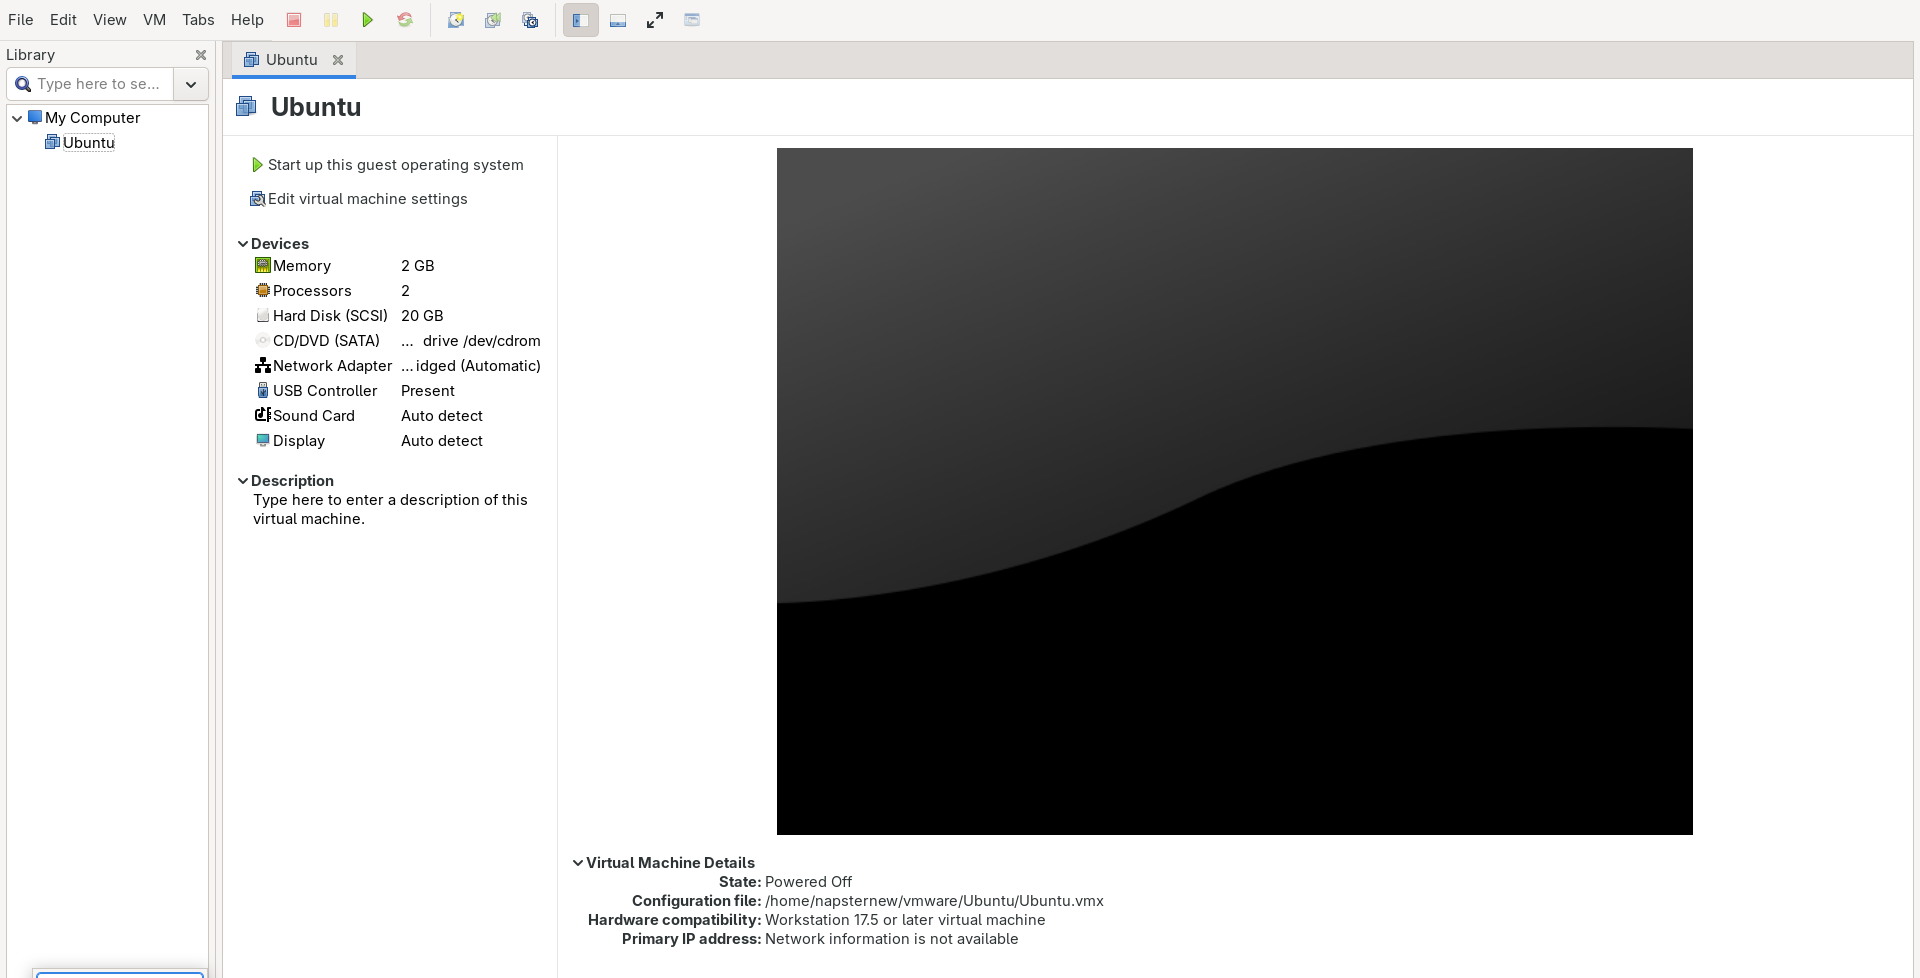
\includegraphics[width=0.9\textwidth]{maquinaVMware6}
  \caption{Máquina virtual configurada en VMware Workstation}
  \label{fig:vm-vmware}
\end{figure}

Luego de comprobar que VirtualBox no funciona correctamente su configuración de red decidimos probar VMware, a su vez para que todos también pudieran tener la misma máquina virtual. Finalmente optamos por KVM, ya que ofrece más opciones de configuración de red, por lo que movimos a KVM tanto el nodo maestro como los nodos de cómputo.

\begin{figure}[H]
  \centering
  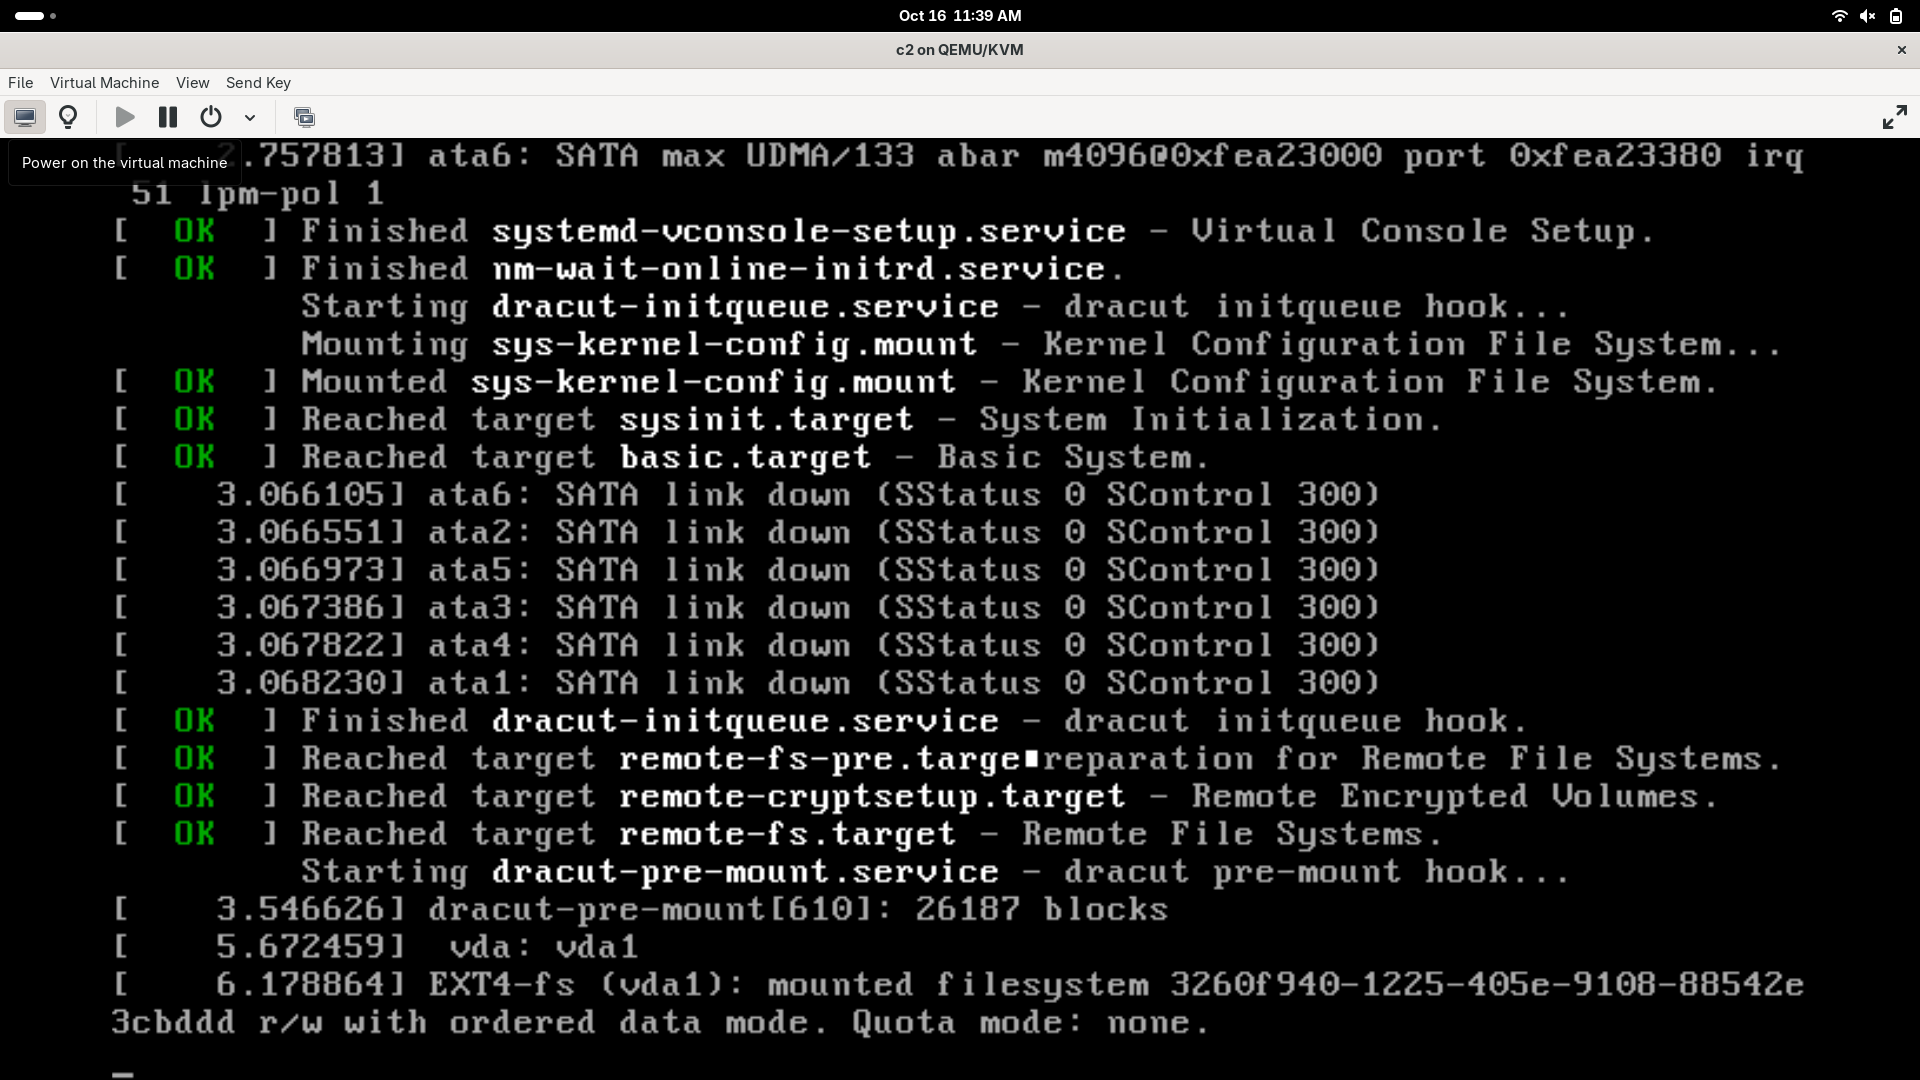
\includegraphics[width=0.9\textwidth]{nodoComputoImagen7}
  \caption{Nodo de cómputo arrancando la imagen por red en QEMU/KVM}
  \label{fig:nodo-imagen}
\end{figure}

Posteriormente Se pudo arrancar el primer nodo de cómputo via ethernet, por lo que decidimos replicar los pasos para poder tener el mismo resultado con los otros 2 nodos restantes.

\begin{figure}[H]
  \centering
  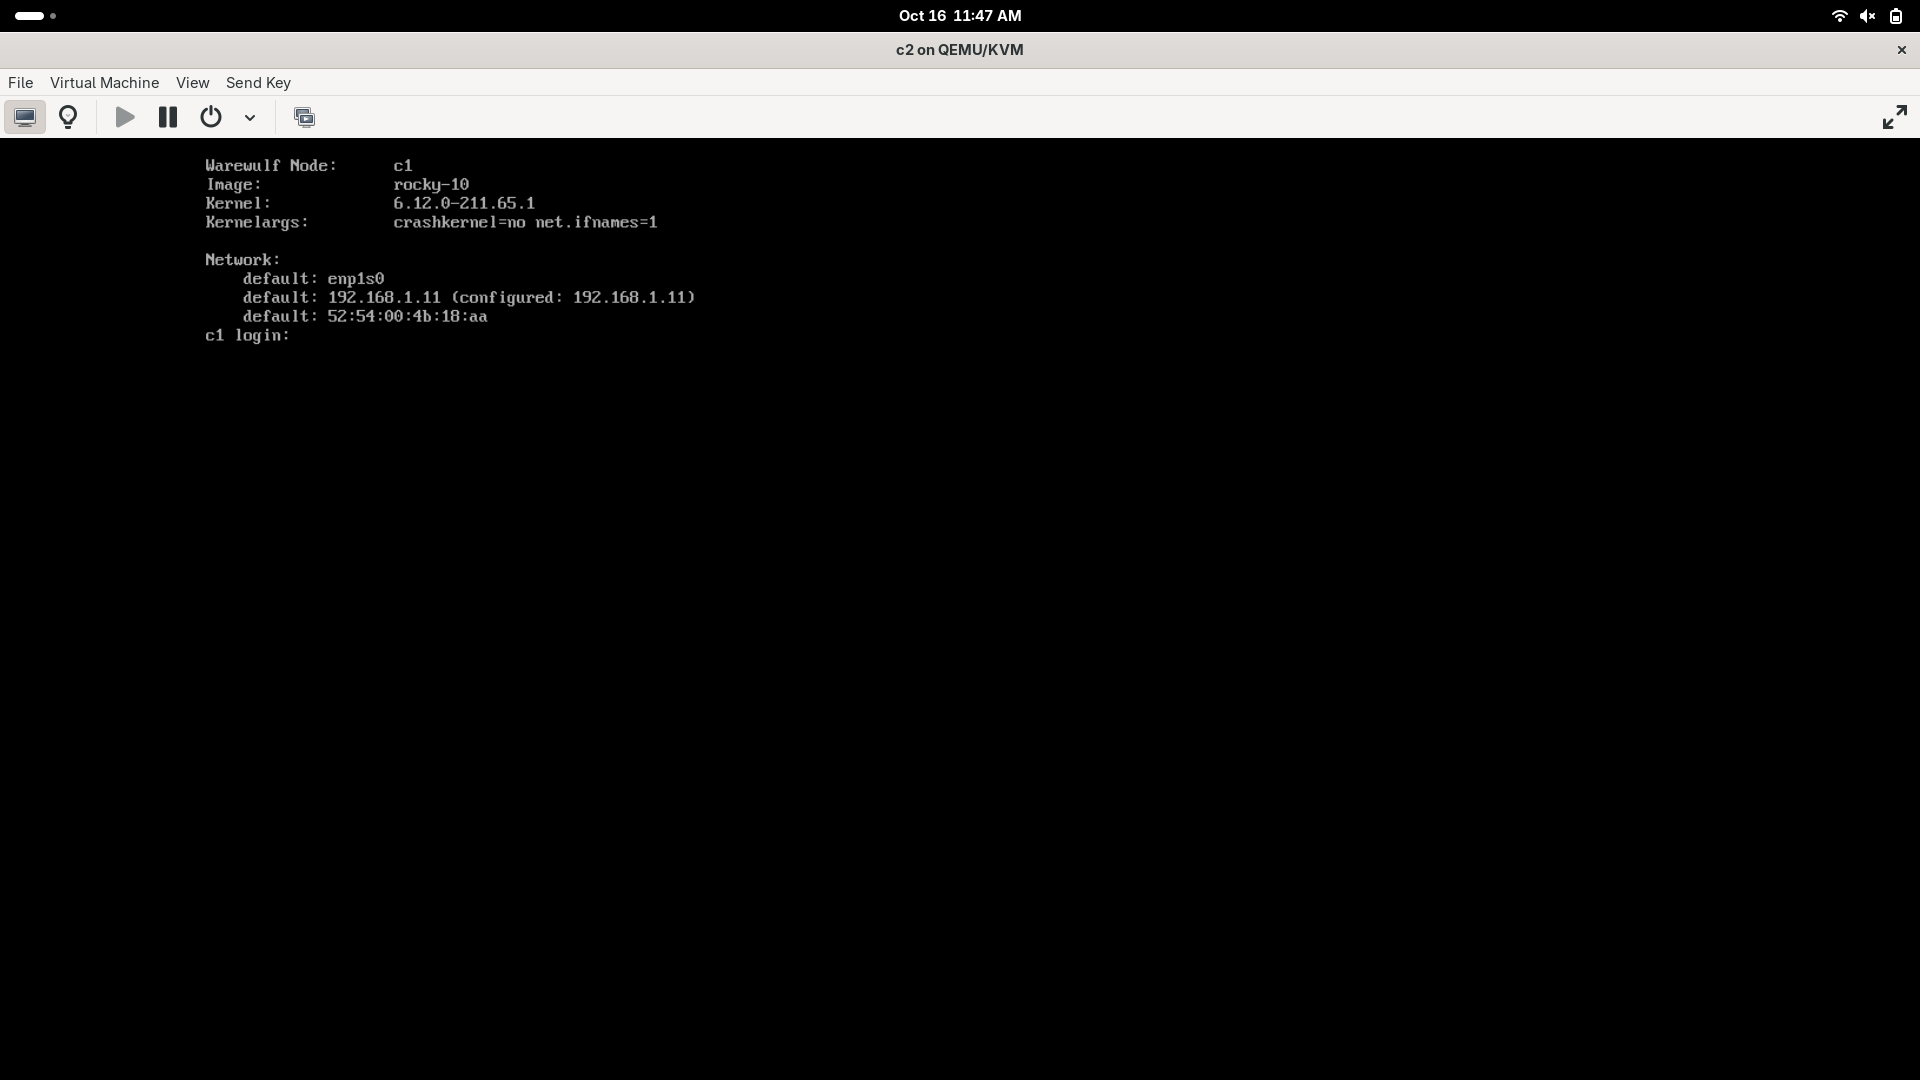
\includegraphics[width=0.9\textwidth]{nodoComputoLogin8}
  \caption{Nodo de cómputo \texttt{c1} con la imagen \texttt{rocky-10} y la dirección \texttt{192.168.1.11} asignada}
  \label{fig:nodo-login}
\end{figure}

Teniendo éxito con el siguiente nodo también, se procedio a hacer login con las credenciales asignadas por el nodo maestro, demostrando que funcionó la instalación y que estabamos a un paso de poder terminar la práctica.

\begin{figure}[H]
  \centering
  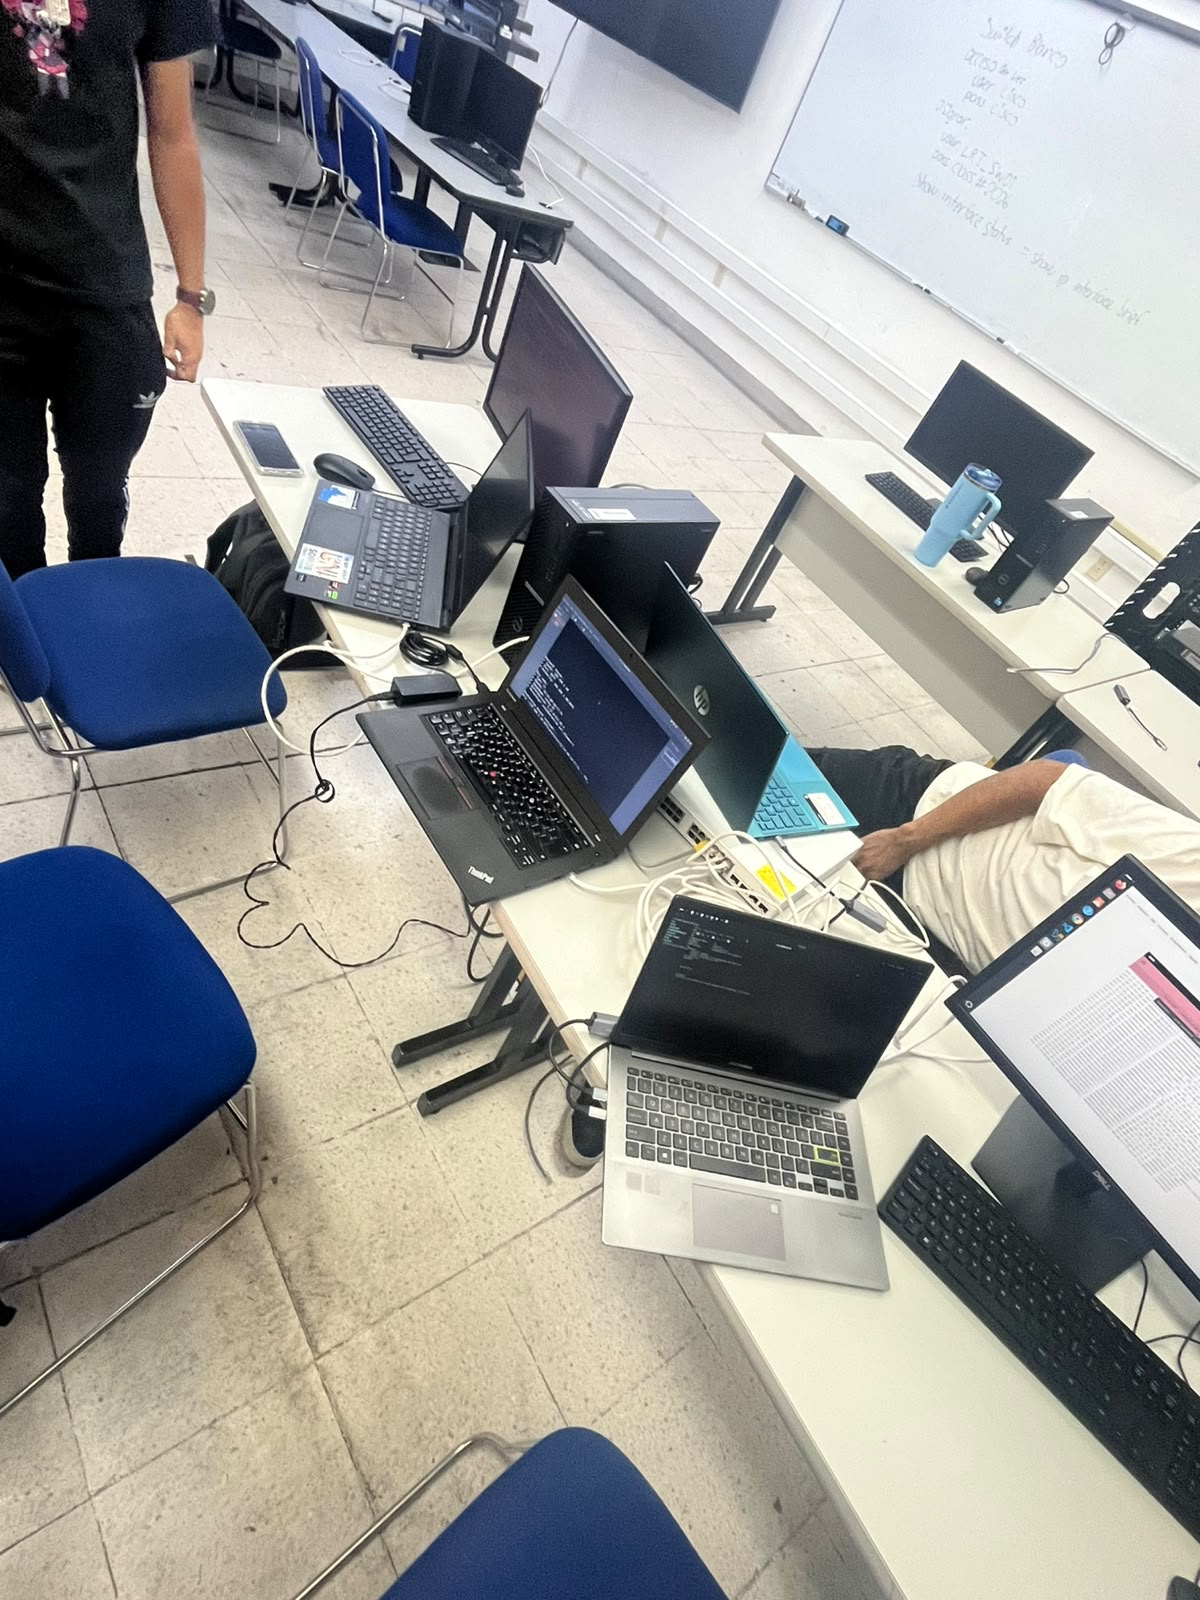
\includegraphics[width=0.5\textwidth]{clusterFisico9}
  \caption{Montaje físico de los equipos del cluster}
  \label{fig:cluster-fisico}
\end{figure}

La \cref{fig:cluster-fisico} muestra el como armamos la topología propupesta ese día, debido a que estabamos fuera de día de práctica optamos por usar un mini switch que funcionaba de la misma forma, también tenemos las 3 laptops funcionando como nodos y el equipo de el salón como nodo maestro.

\begin{figure}[H]
  \centering
  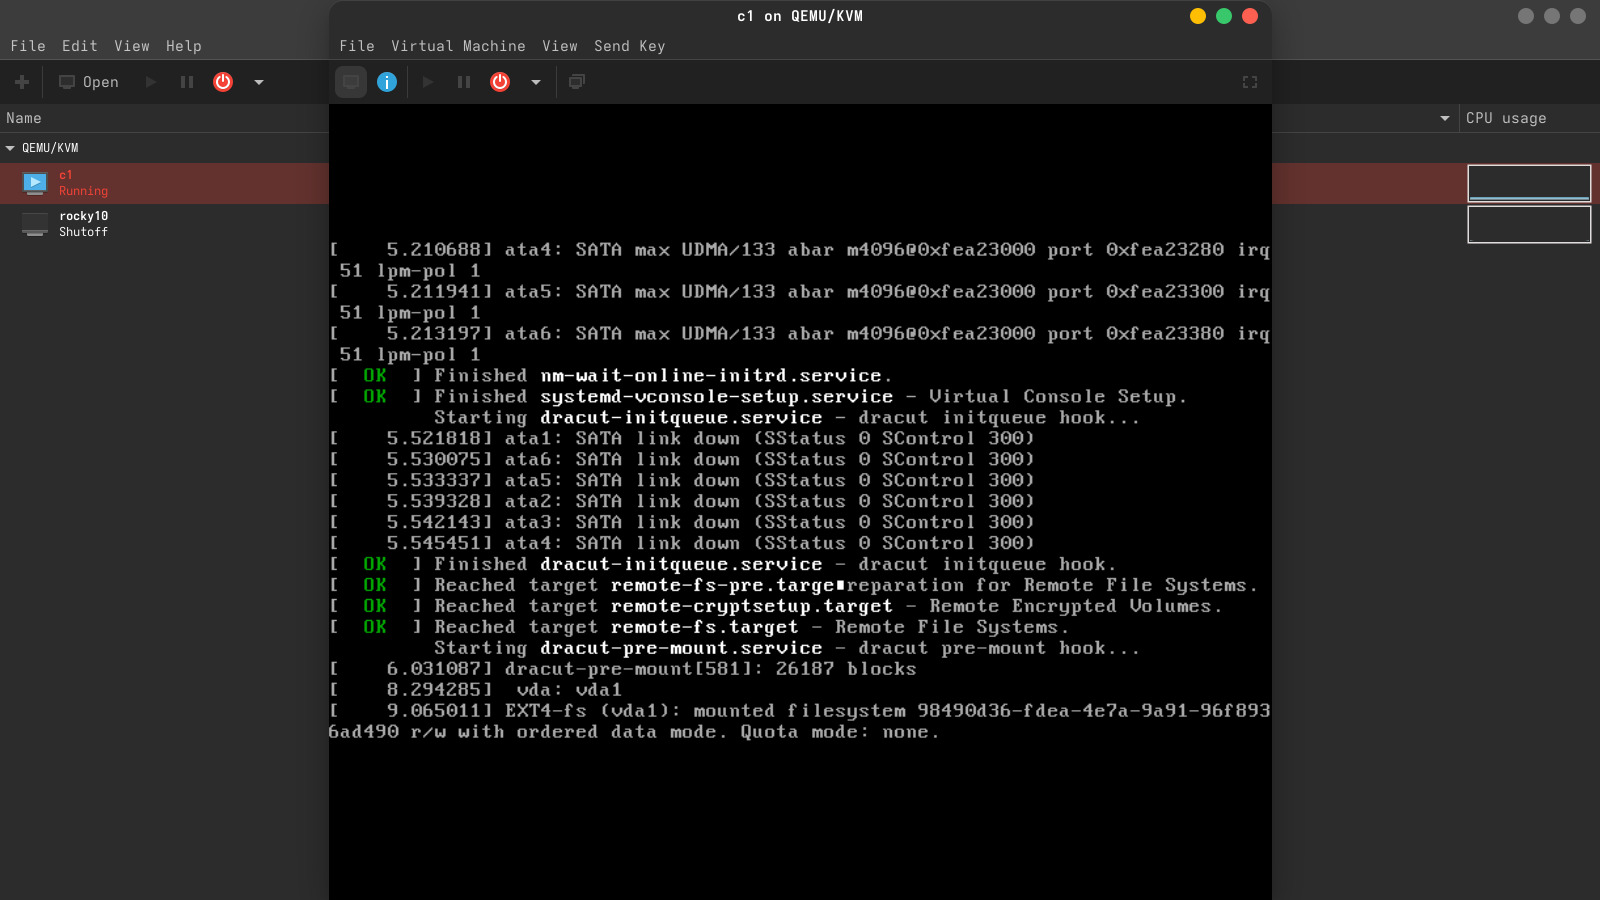
\includegraphics[width=0.9\textwidth]{nodoComputoIniciando10}
  \caption{Arranque del nodo de cómputo \texttt{c1} por red}
  \label{fig:nodo-arranque}
\end{figure}

Finalmente el último nodo de cómputo inicio por red, de igual forma de manera éxitosa y con las credenciales asignadas.

\begin{figure}[H]
  \centering
  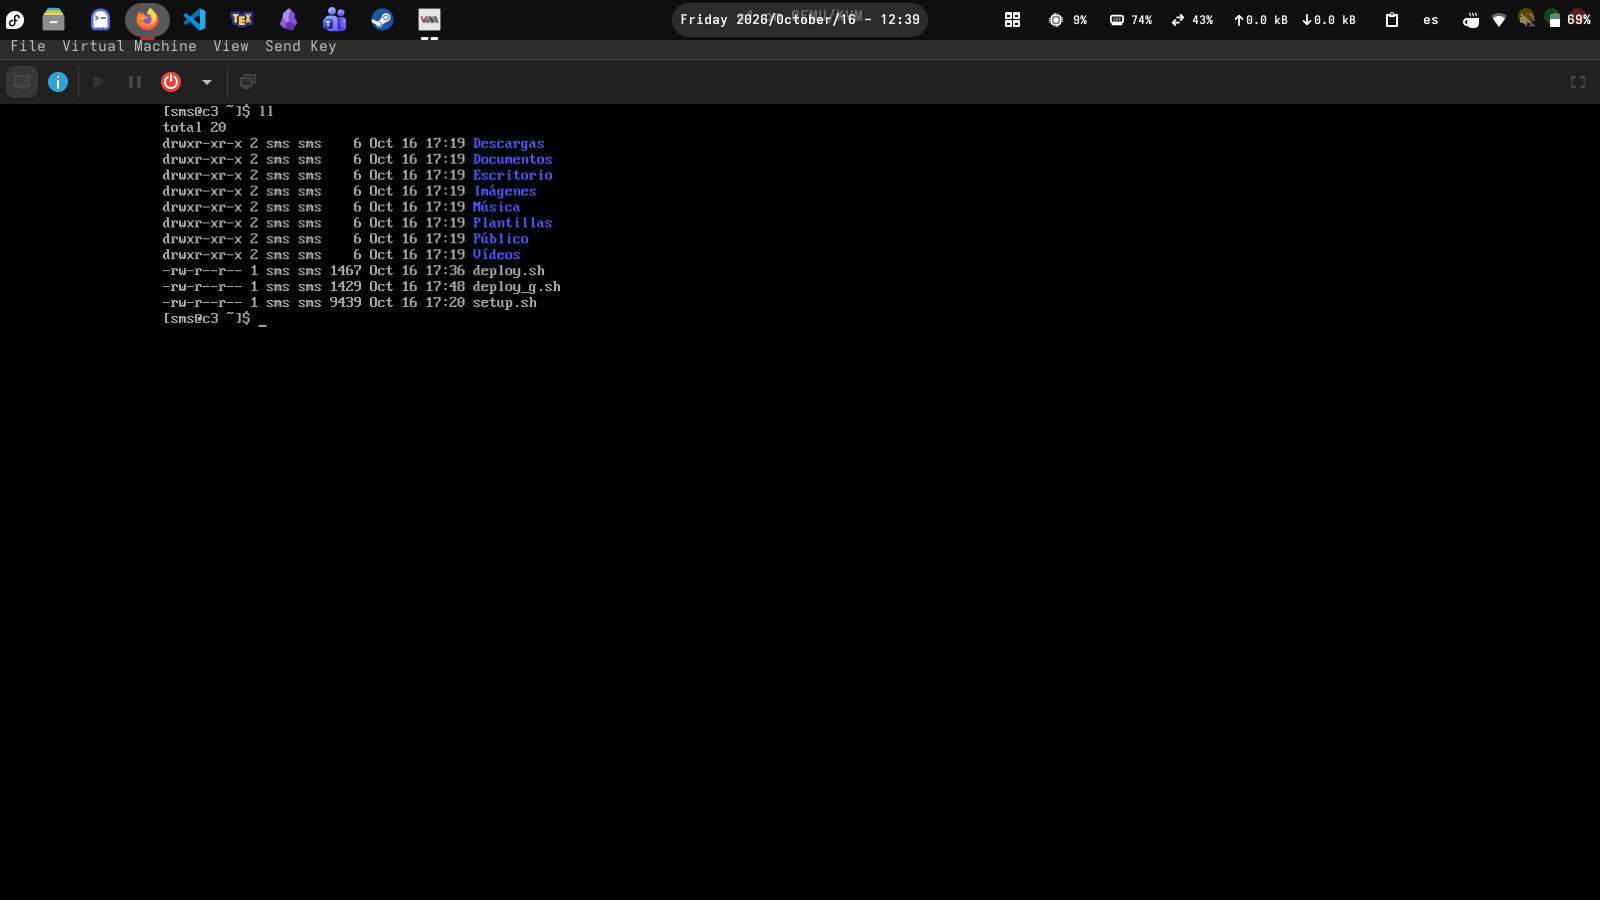
\includegraphics[width=0.9\textwidth]{nodoComputoSMS11}
  \caption{Sesión iniciada en el nodo de cómputo \texttt{c3}}
  \label{fig:nodo-sesion}
\end{figure}

De la misma forma que la imagen anterior, el nodo de cómputo número tres ya esta funcionando con su dirección asignada e incluso con sesión ya iniciada con sus credenciales asignadas.

\begin{figure}[H]
  \centering
  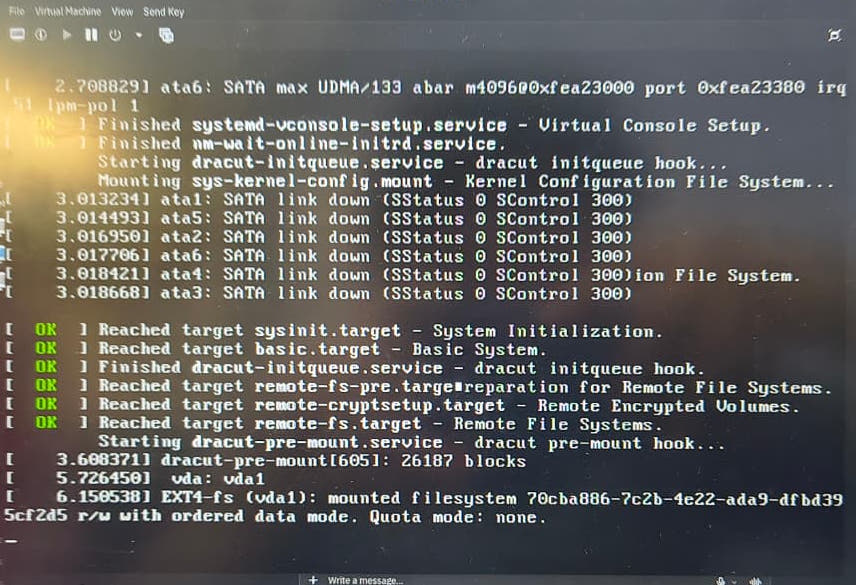
\includegraphics[width=0.9\textwidth]{nodoMaestroIniciando12}
  \caption{Arranque de la imagen por red en un equipo del cluster}
  \label{fig:maestro-arranque}
\end{figure}

Como penúltimo detalle, esta también fue una parte en la que a veces los nodos de cómputo se quedaban congelados sin avanzar ya con rocky 10 booteado por red.

\begin{figure}[H]
  \centering
  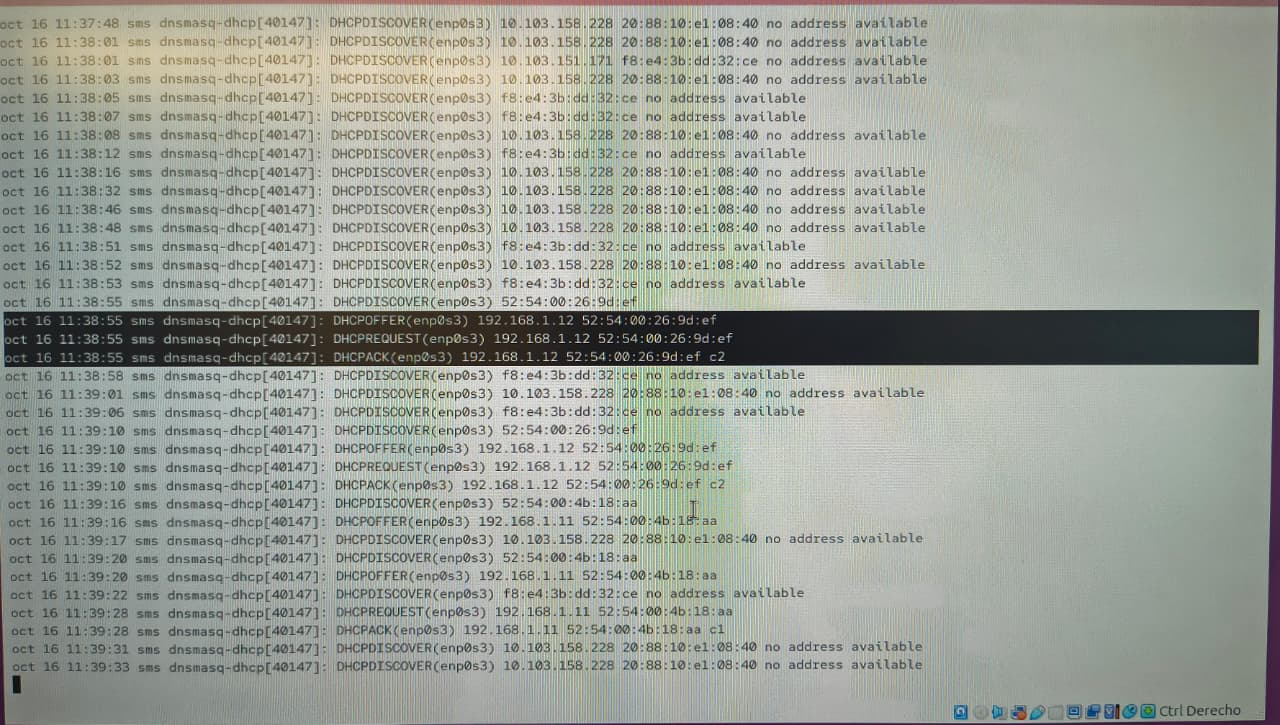
\includegraphics[width=0.9\textwidth]{nodoMaestroDHCP13}
  \caption{Registro del servidor DHCP del nodo maestro asignando direcciones a los nodos de cómputo}
  \label{fig:maestro-dhcp}
\end{figure}

Por último, se demuestra con la \cref{fig:maestro-dhcp} que el nodo maestro asignaba las direcciones y los nodos de cómputo las aceptaban, teniendo por fin los 3 nodos funcionando correctamente.
\section{Conclusiones}
\label{sec:conclusiones}

Siguiendo la guía de OpenHPC 4.1 para Rocky Linux 10 con Warewulf y Slurm, logramos instalar el nodo maestro y preparar los nodos de cómputo sobre máquinas virtuales. Al nodo maestro se le instaló el sistema operativo base con SELinux deshabilitado, el servidor NTP, los componentes de OpenHPC, el servidor de Slurm y Warewulf. A partir de él se generó la imagen \texttt{rocky-10} que reciben los nodos de cómputo.

El objetivo principal se cumplió en parte. Los nodos de cómputo llegaron a arrancar por red con la imagen distribuida por Warewulf y recibieron la dirección que les correspondía en la red privada, como muestran la \cref{fig:nodo-login} y la \cref{fig:maestro-dhcp}. Sin embargo, no alcanzamos a ejecutar a tiempo la prueba del hola mundo con MPI, por lo que no pudimos comprobar que el cluster ejecute trabajos en paralelo a través de Slurm.

La mayor dificultad estuvo en la red y no en la instalación de los paquetes. Durante varios intentos el servidor DHCP del nodo maestro ofrecía la dirección a cada nodo, pero estos la rechazaban y no arrancaban la imagen por red, incluso con la dirección asignada manualmente. De esto concluimos que en un cluster y la configuración de las interfaces, del direccionamiento de la red privada y del servicio DHCP debe quedar perfectamente configurado ya que si no atrasa bastante la instalación del Cluster debido a que sin red no hay comunicación entre los nodos ni imagen para los mismos.

Trabajar con máquinas virtuales nos permitió repetir la instalación y probar varios programas de virtualización (VirtualBox, KVM y VMware), aunque cada uno maneja de forma distinta los adaptadores de red, y eso influye directamente en el arranque por red de los nodos, gracias a esto terminamos optando por KVM ya que tiene más opciones de configuración de red.

\subsection{Conclusiones personales}
Mauricio:
El haber realizado la instalación de Rocky y del nodo maestro en VirtualBox más aparte haber tenido que realizar llaves y firmarlas debido a problemas entre el kernel y el mismo software nos atrase mucho más de lo que debimos de haber tardado, finalmente ya que cambiamos a software que era VMware fue más fácil la instalación y como ya conocía el proceso de firmar las llaves del kernel fue más ágil, pero aún así no conseguí que funcionará ni como nodo maestro ni como nodo de cómputo con el nodo maestro que ya funcionaba de KVM, y fue por ello que mejor entre todo el equipo nos movimos a KVM ya que en fedora es mucho más configurable y fácil de manejar que todos los softwares anteriores, siendo este último el único que funciono y sin muchas trabas fuera del mismo problema del DHCP, considero que hubieramos terminado a tiempo si hubieramos tenido softwares ya definidos como para no hacer prueba y error.
\\[1em]
Jacobo:
Tres de los cuatro integrantes del equipo contamos con el sistema operativo de Fedora, por lo que al inicio tuvimos algunas dificultades con el software de Virtualbox por lo que finalmente decidimos usar QEMU/KVM en su lugar ya que al parecer este software esta mejor optimizado para este S.O. en especifico, sin embargo esto también nos trajo algunos problemas, el principal fue la conexion Ethernet ya que era algo mas difícil usar adaptadores tipo pueden en las VM, sin embargo al final pudimos resolver este problem usando una NIC MacVTap.
Finalmente puedo decir que esta practica fue posiblemente una de las mas difíciles a las que me he enfrentado dado que es necesario tener conocimientos en Linux con sistemas Red Hat como lo es Rocky, ademas de conocimientos básicos en redes, pero no lo normal si no precisamente en temas básicos como lo son los tipos de interfaces: NAT, puente, etc y finalmente conocimientos básicos sobre maquinas virtuales. Sin duda este experimento me trajo muchos conocimientos que estoy seguro aplicare en proyectos futuros.
\\[1em]
Francisco:
La realización de este proyecto me permitió comprender mejor el proceso de configuración e implementación de un clúster, así como las dificultades que pueden presentarse durante su desarrollo. A lo largo del proyecto surgieron diversos problemas relacionados con las máquinas virtuales, la configuración de las interfaces de red, la instalación de herramientas y la comunicación entre los nodos. A pesar de los intentos realizados y de las diferentes soluciones que se investigaron, no fue posible establecer la conexión final del clúster. Sin embargo, considero que esta experiencia fue importante para mi aprendizaje, ya que me permitió desarrollar habilidades para identificar errores, investigar posibles soluciones y comprender la importancia de realizar cada configuración correctamente. Personalmente, aprendí que este tipo de proyectos requiere paciencia, tiempo, organización y trabajo en equipo. Aunque no se logró cumplir completamente el objetivo, los conocimientos adquiridos durante el proceso representan una base útil para futuros proyectos, en los que podré aplicar lo aprendido y enfrentar problemas similares con mayor experiencia y preparación.
\\[1em]
Guillermo:
La implementación del clúster con OpenHPC y Rocky Linux fue un desafío complejo pero muy interesante. Quedó claro que una mejor planeación inicial habría agilizado considerablemente nuestro avance. Interconectar varias máquinas virtuales es complicado, y lidiar con los distintos sistemas y configuraciones en la PC de cada integrante lo dificultó más. Lo ideal sería estandarizar el entorno para todos, partiendo de una instalación de sistema operativo desde cero.
En mi caso, instalaciones previas de Docker requirieron ajustes extra para lograr tener red en la máquina virtual. A esto se suma que el manual oficial es excesivamente técnico y asume muchos pasos y comandos de configuración. Finalmente, tras la experiencia, creo que existen distribuciones basadas en Red Hat más adecuadas que Rocky Linux para este tipo de implementaciones.

\section{Bibliografía}
\label{sec:bibliografía}

Rocky Linux. (s. f.-b). Rocky Linux. https://rockylinux.org/download 
\\
OpenHPC. (2026). OpenHPC (v4.1) Cluster Building Recipes. En OpenHPC.
https://github.com/openhpc/ohpc/releases/download/v4.1.GA/openhpc_4.1-install_guide-rocky10-warewulf-slurm-x86_64.pdf




% --- Bibliografia ---------------------------------------------------
\printbibliography[heading=bibintoc, title={Referencias}]

% --- Indices opcionales (descomentar si se usan) --------------------
% \listoffigures
% \listoftables

\end{document}
